\pdfminorversion=4
\documentclass[aspectratio=169]{beamer}
\usepackage{verbatim}
\newenvironment{metaverbatim}{\verbatim}{\endverbatim}
\usepackage{courier}
\usepackage{lmodern}
\usepackage{apacite}
\usepackage[hidelinks]{hyperref}
\usepackage{xcolor}
\xdefinecolor{azulcesafuerte}{HTML}{14387e}
\xdefinecolor{azulcesaclaro}{HTML}{7ab6e0}
\xdefinecolor{azulcesamedio}{HTML}{0A72BC}

\usetheme{Madrid}
%\usecolortheme[named=black]{structure}
%
\setbeamercolor{normal text}{fg=azulcesafuerte}
\setbeamercolor{background canvas}{bg=white}
\setbeamercolor{frametitle}{fg=white, bg=azulcesafuerte}
\setbeamercolor{block title}{bg=azulcesafuerte,fg=azulcesaclaro}
\setbeamercolor{navigation symbols}{}

\setbeamertemplate{background}{\tikz[overlay,remember picture]\node[opacity=0.15]at (current page.center){\includegraphics[width=6.5cm]{}};}
\usepackage{tikz}
\usepackage{kantlipsum}
\setbeamercolor*{title}{fg=white, bg=azulcesafuerte}
\setbeamercolor{titlelike}{parent=structure}

\setbeamercolor*{palette primary}{bg=azulcesafuerte,fg=white}
\setbeamercolor*{palette secondary}{bg=azulcesafuerte,fg=white}
\setbeamercolor*{palette tertiary}{bg=azulcesafuerte,fg=white}

% Change base colour beamer@blendedblue (originally RGB: 0.2,0.2,0.7)
\colorlet{beamer@blendedblue}{azulcesaclaro}
\usepackage[english]{babel}
\usepackage{apacite}
\usepackage{marvosym}
\usepackage{subfig}
\usepackage{graphicx}
\usepackage[utf8x]{inputenc}
\usepackage{url}
\usepackage{hyperref}
\usepackage{times}
\usepackage{pxfonts}
\usepackage{fontenc}
%\usepackage[dvipsnames]{xcolor}
\setbeamertemplate{bibliography item}[text]
\title[Fundamentos de Analítica de Datos: Caso 1]{Fundamentos de Analítica de Datos: Caso 1}
\subtitle{(Sesión 6A)}

\author[Prof. Juan C. Correa, Ph.D.]{Prof. Juan C. Correa, Ph.D.}

\institute[]{
Colegio de Estudios Superiores de Administración\\
Bogotá - Colombia\\
% \color{azulcesaclaro}\Email  \href{mailto:juan.correan@cesa.edu.co}{juan.correan@cesa.edu.co}
}
\pgfdeclareimage[height=0.6cm]{OL}{OL}
 \logo{\pgfuseimage{OL}}
 \setbeamertemplate{caption}[numbered]
\date[Bogotá, Agosto, 2021] % (optional)
{}

\subject{}
\begin{document}
\begin{frame}
\titlepage
\end{frame}

% \begin{frame}
% \frametitle{Agenda} 
% \tableofcontents
% \end{frame}

\begin{frame}
\begin{block}{Objetivo de Aprendizaje}
En la Sesión 4B, se presentó un artículo sobre las entregas de comida a domicilios en Bogotá y se usaron sus datos para aprender algunas técnicas sencillas de visualización de datos. Al finalizar esta sesión, usted comprenderá el por qué y para qué del pre-procesamiento y la visualización de datos.
\end{block}
\end{frame}

\section{Insumos Preliminares}
\begin{frame}
\begin{center}
\Huge
\textcolor{azulcesaclaro}{1\\
--------------------------------\\
Insumos Preliminares}
\end{center}
\end{frame}

\begin{frame}
Para esta sesión, usted debe usar GitHub Desktop para clonar el siguiente repositorio.
\begin{figure}
\centering
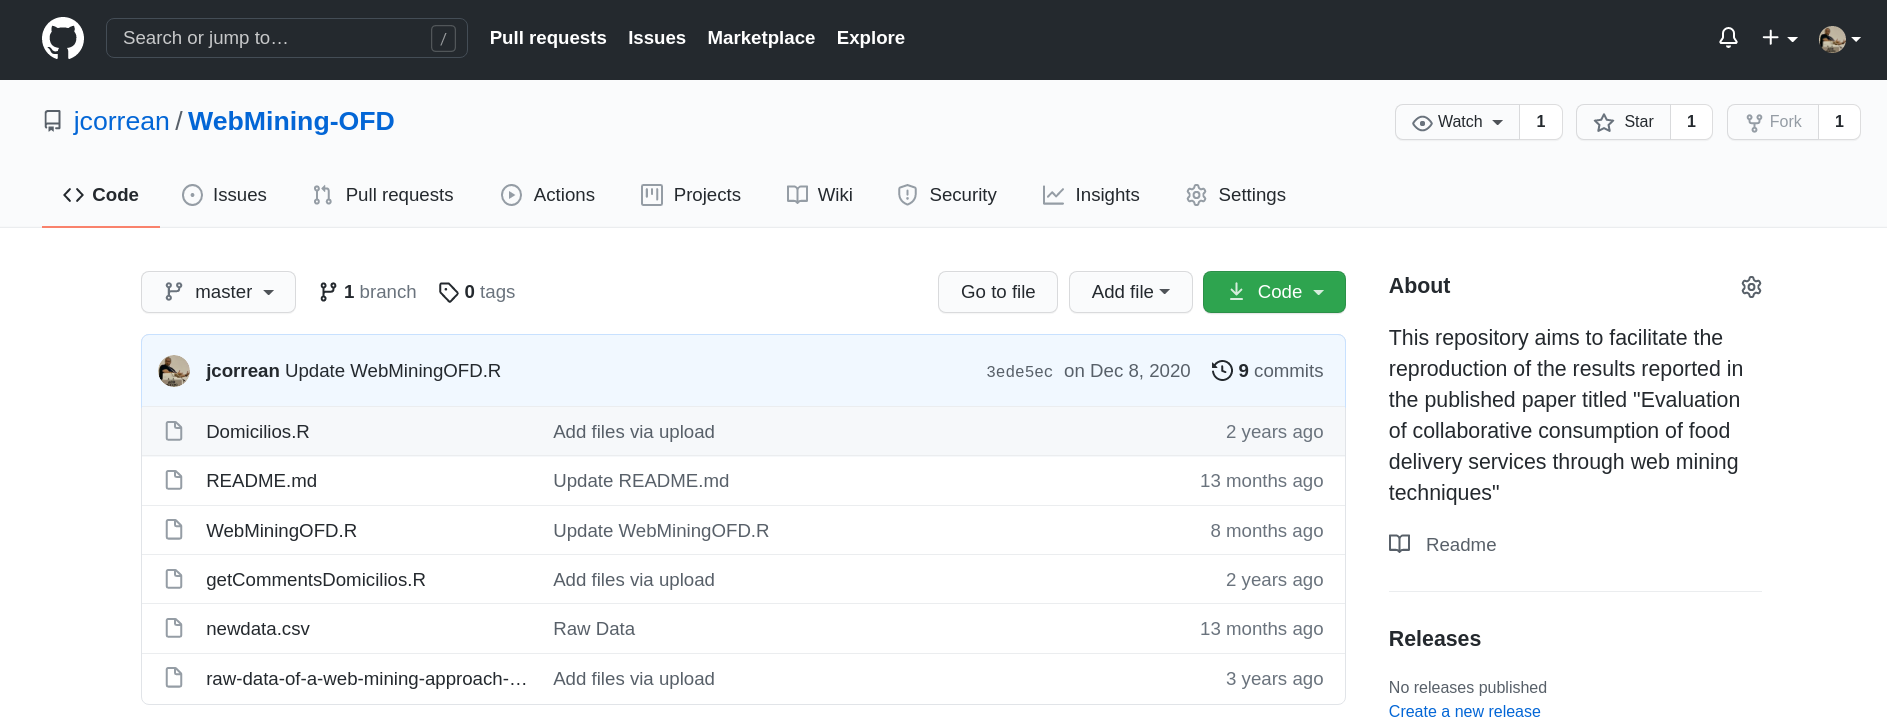
\includegraphics[width=.85\textwidth]{github1.png}
\end{figure}
\centering
\textcolor{blue}{\url{https://github.com/jcorrean/WebMining-OFD}}
\end{frame}

\section{Fundamentos de Pre-procesamiento de Datos}
\begin{frame}
\begin{center}
\Huge
\textcolor{azulcesaclaro}{2\\
--------------------------------\\
Fundamentos de Pre-procesamiento de Datos}
\end{center}
\end{frame}

\begin{frame}
En la sesión 3B (slide 10) afirmamos que las bases de datos ideales son aquellas que ya se encuentran listas para ser usadas para analizar los datos estadísticamente.\\
\vspace{0.5cm}
\textbf{El pre-procesamiento de datos} comprende a todas las herramientas y actividades que deben hacerse luego de haber recolectado los datos y antes de analizarlos. 
\begin{figure}
\centering

\includegraphics[width=.5\textwidth]{tools.png}
\end{figure}
\end{frame}

\begin{frame}
\begin{figure}
\centering

\includegraphics[width=.8\textwidth]{tidy.png}
\end{figure}
\end{frame}

\begin{frame}
Demostración de Pre-Procesamiento con R
\begin{figure}
\centering
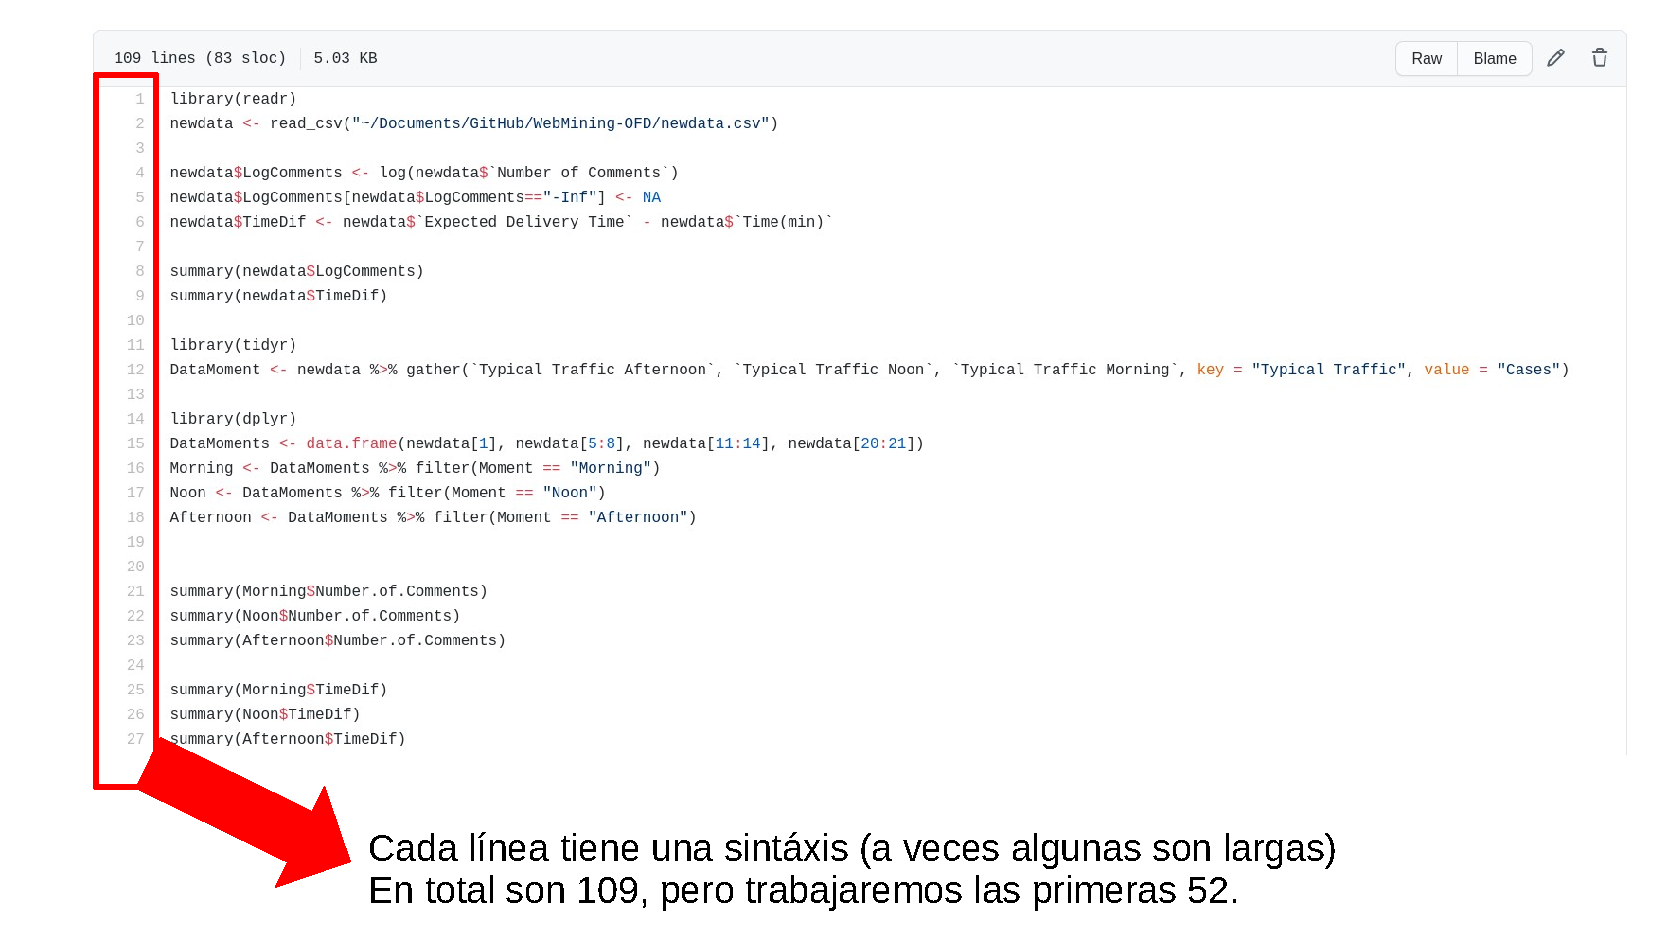
\includegraphics[width=.8\textwidth]{Ejercicio6A.pdf}
\end{figure}
\end{frame}

\begin{frame}
Ejercicio guiado:\\
\vspace{0.3cm}
En este ejercicio, una vez visto el ejemplo de pre-procesamiento que se realizó en R, vamos a intentar desarrollar nuestro primer código de Python. \\
\vspace{0.3cm}
Vamos a abrir un jupyter Notebook para comprender las siguientes  sintaxis desarrolladas en lenguaje R y escribir sus equivalentes en Python:\\
\begin{itemize}
\item[1] \texttt{library(readr)}  (línea 1 del repo GitHub)
\item[2] \texttt{newdata <- read\_csv('direccion/discoduro/donde/esta/el/archivo.csv')} (línea 2 del repo GitHub)
\item[3] \texttt{newdata\$LogComments <- log(newdata\$\`~Number of Comments\`~)}
\end{itemize}
\vspace{0.3cm}
La sintaxis 3 genera una nueva columna en la base de datos \texttt{newdata} llamada \texttt{LogComments} que es el resultado de calcularle el logaritmo a la variable  \`~Number of Comments\`~
\end{frame}

\begin{frame}
Para cumplir con el ejercicio guiado (y como futuros directivos de una empresa data-driven), hay que entender cómo trabaja un experto en analítica de datos. Eso supone ponerse en sus zapatos y asumir el desafío de documentarse.
\begin{figure}
\centering

\includegraphics[width=.7\textwidth]{Desafios.png}
\end{figure}
\end{frame}

\begin{frame}
Algunas pistas:
Recordando brevemente, la definición del término \textbf{datos} es el registro alfanumérico de una o más observaciones de un fenómeno. Los datos en Python tienen varios nombres según sus características
\vspace{0.5cm}
\begin{figure}
\centering
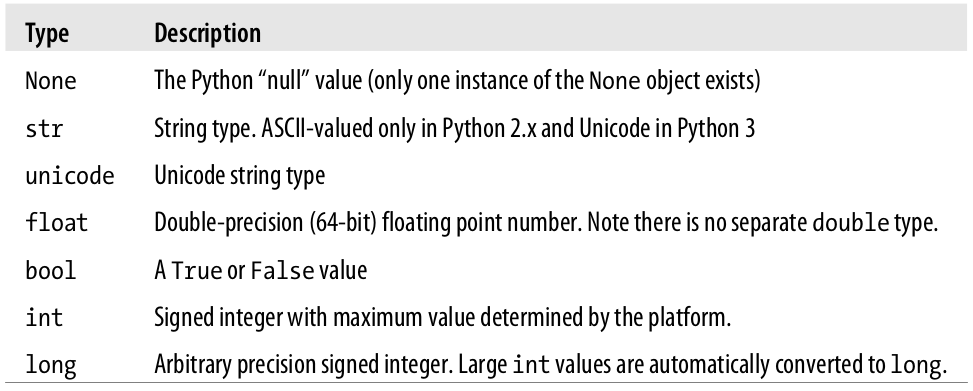
\includegraphics[width=.8\textwidth]{ScalarType.png}
\end{figure}
\end{frame}

\begin{frame}
En analítica de datos, los datos tienen una estructura computacional específica. Las estructuras de los datos en Python son:
\begin{itemize}
\item Tuple
\item List
\item Dict
\item Set
\item Index
\item Series
\item DataFrames
\end{itemize}
De todas estas estructuras, quizás las más frecuentes son List y DataFrame
\end{frame}

\begin{frame}
Una Tuple y una List son colecciones o secuencias de objetos. La Tuple es una colección inmutable y fija de objetos. La List es una colección mutable y variable de objetos. Ejemplos:\\
\vspace{0.5cm}
\texttt{Tuple = 4, 5, 6}\\
\texttt{List = [4, 5, TRUE, 'Hola']}\\
\vspace{0.5cm}
Los DataFrames son tablas tipos hojas de excel en las que se tiene un colección ordenada de columnas, cada una de las cuales puede contener sus propias características (número entero, número con decimales, booleano, alfanumérico, etc.). Los dataframes tienen indices para sus columnas y filas
\end{frame}

% \begin{frame}
% \begin{figure}
% \centering
% 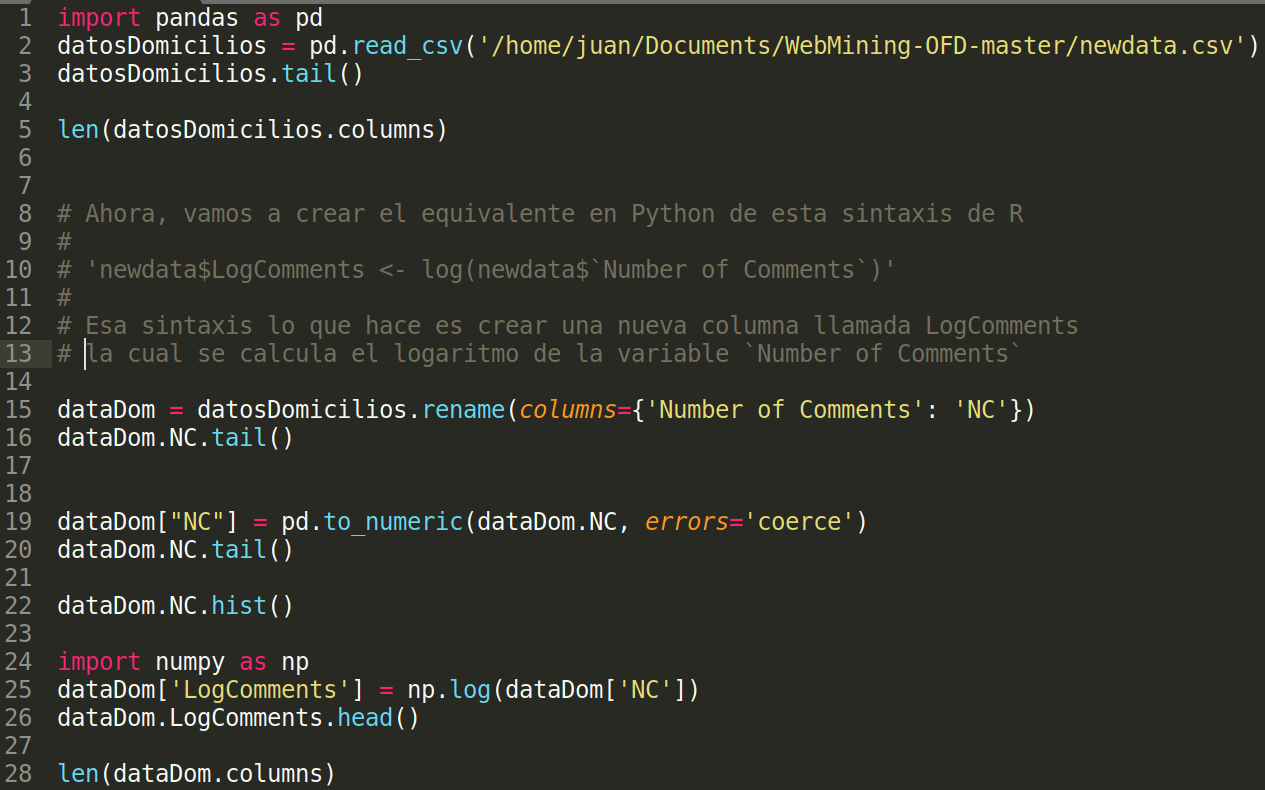
\includegraphics[width=.8\textwidth]{script.png}
% \end{figure}
% \end{frame}

\section{Fundamentos de Visualización de Datos}
\begin{frame}
\begin{center}
\Huge
\textcolor{azulcesaclaro}{2\\
--------------------------------\\
Fundamentos de Visualización de Datos}
\end{center}
\end{frame}

\begin{frame}
\begin{figure}
\centering
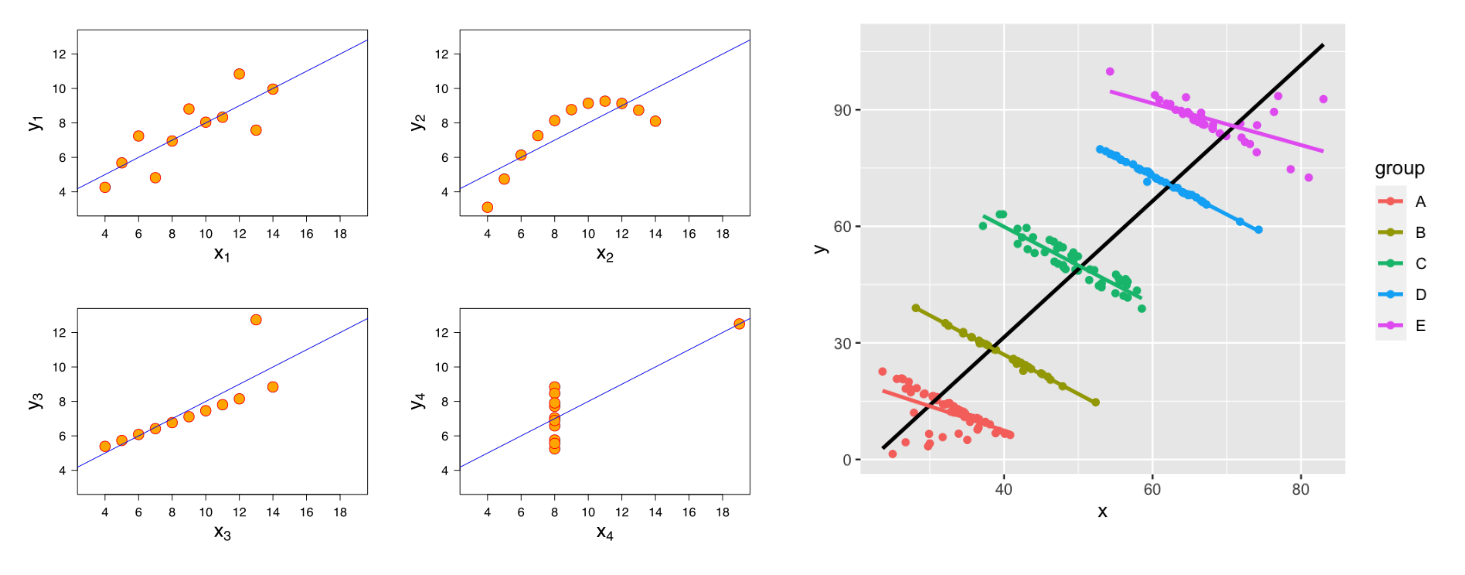
\includegraphics[width=.8\textwidth]{visualization.png}
\end{figure}
El \textbf{Cuarteto de Anscombe} y la \textbf{Paradoja de Simpson} son dos casos que ilustran el valor fundamental de aprender a usar las técnicas de visualización estadística como herramienta indispensable para la comunicación de información y conocimiento.
\end{frame}

\begin{frame}
\begin{figure}
\centering
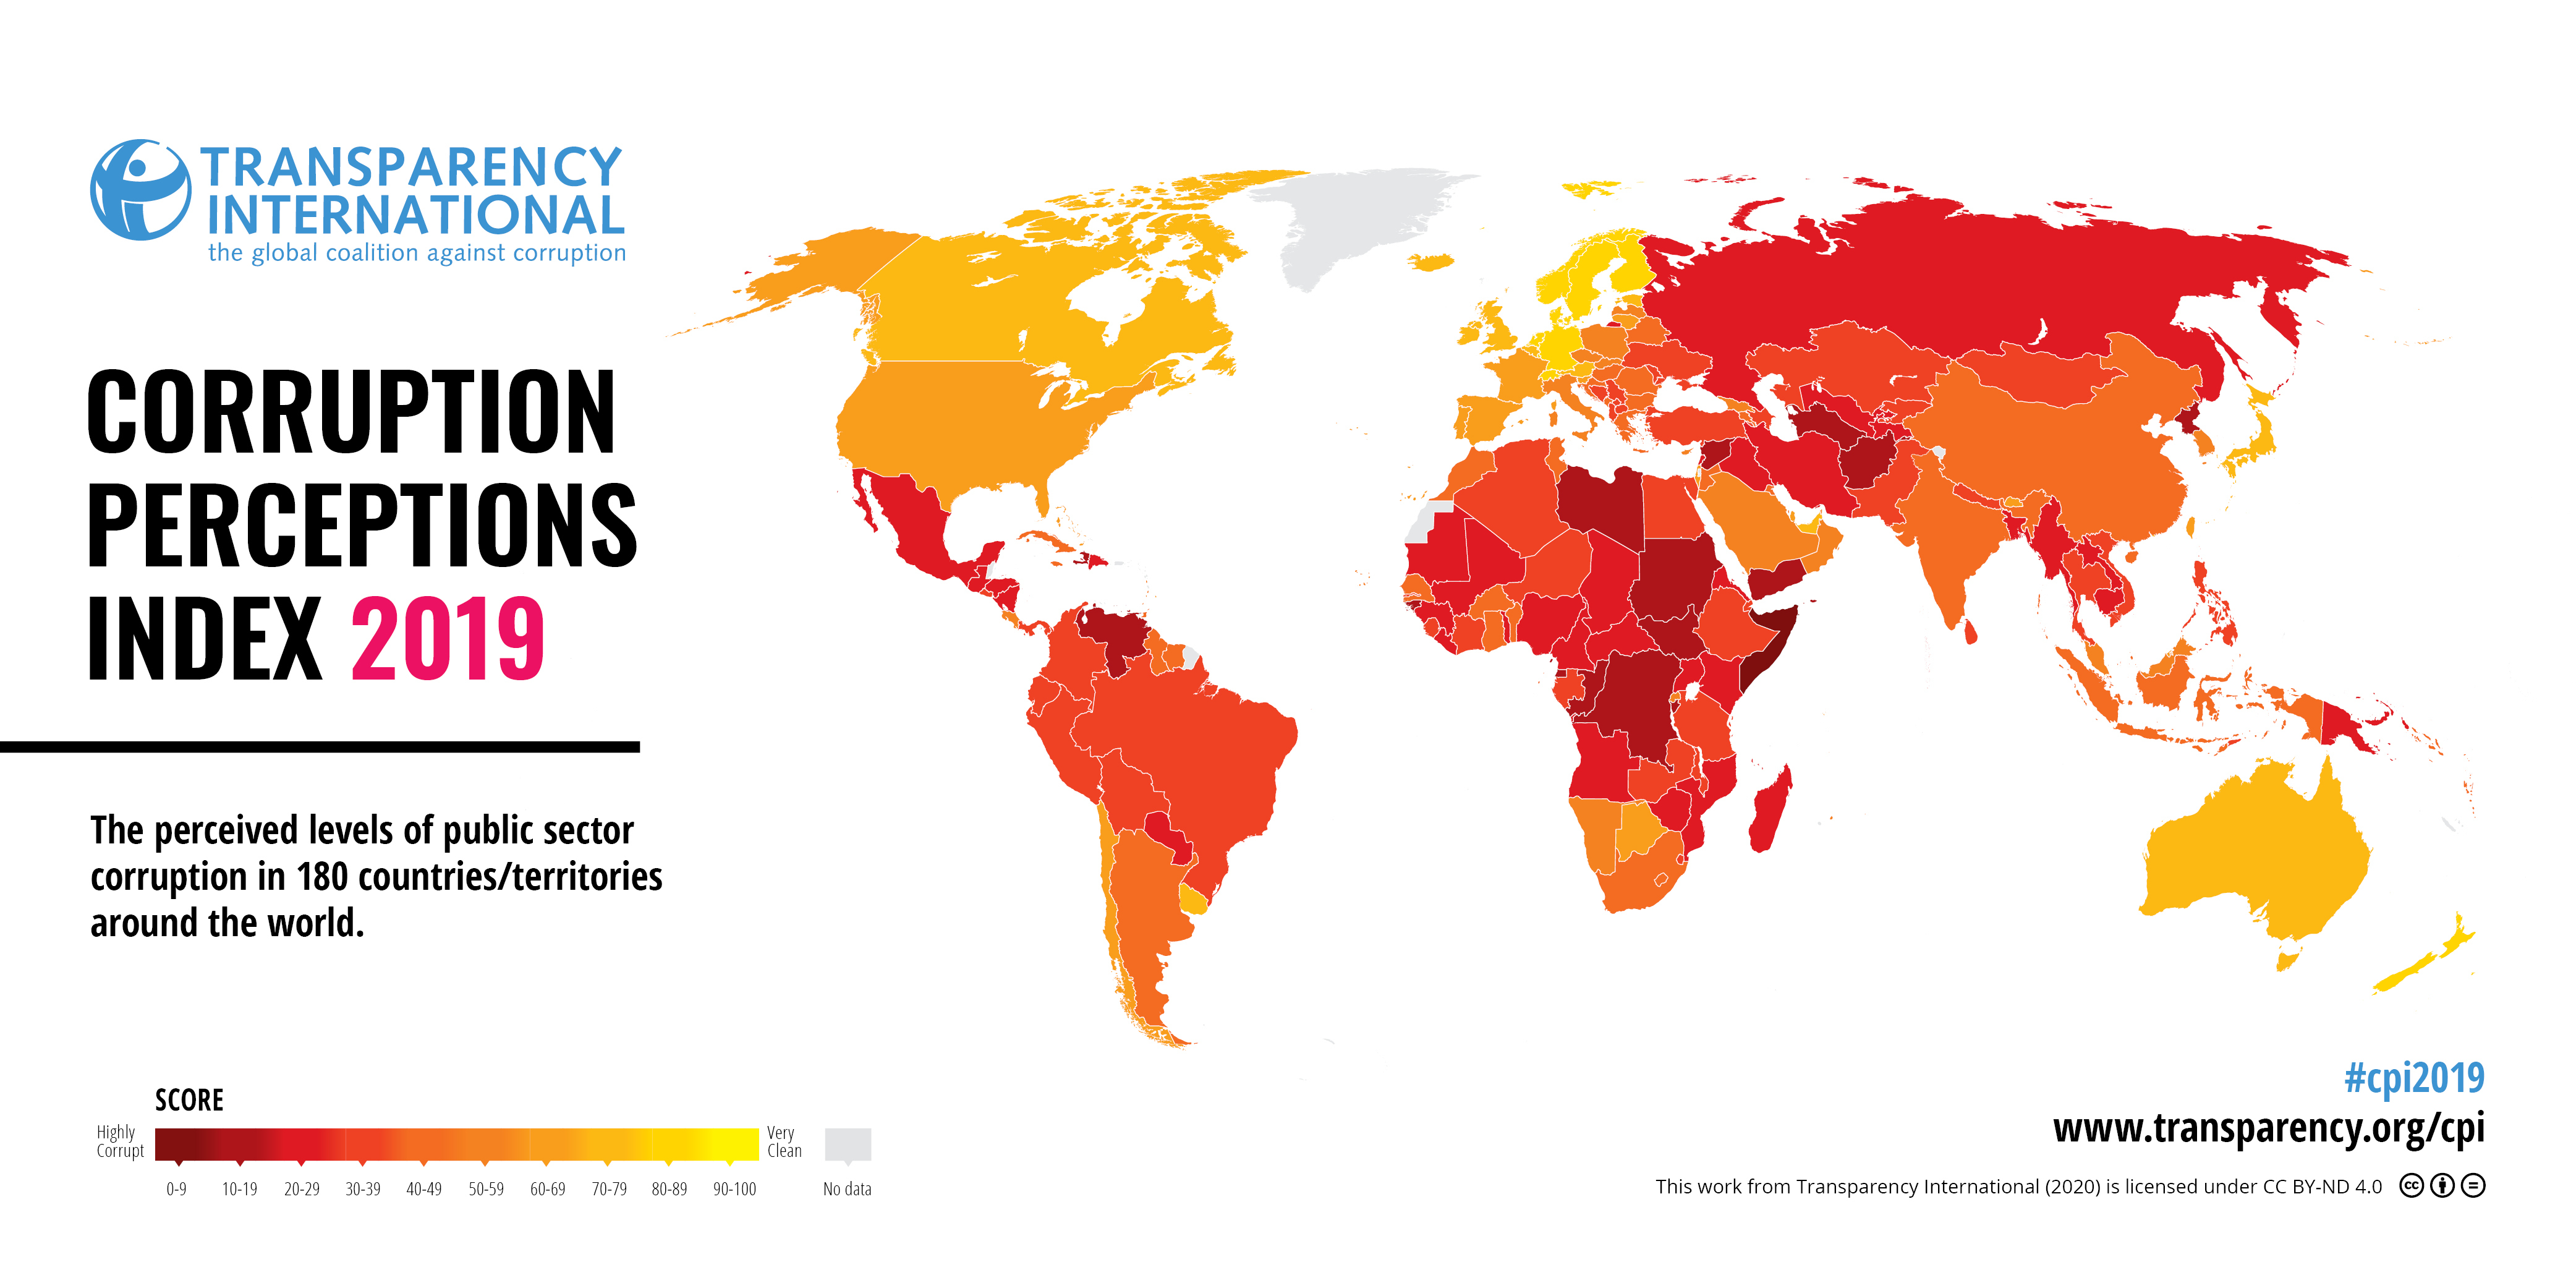
\includegraphics[width=.8\textwidth]{Map.jpg}
\end{figure}
Si se quisiera reflejar esta información en una tabla con datos...\\
¿Cuál sería el aspecto de dicha tabla?
\end{frame}

\begin{frame}
% \Large
Comencemos por conocer las distintas formas de \textbf{presentar información en un reporte gerencial} y comparemos cuál de ellas facilitan la comprensión del lector.\\ 
\vspace{0.3cm}\\
\begin{itemize}
    \item Prosa o texto (Indispensable)
    \item Ecuación 
    \item Tablas
    \item Gráficos estadísticos
    \item Algoritmo computacional
\end{itemize}
\vspace{0.3cm}\\
Para el \textbf{lector promedio}, el formato más fácil de comprender es aquel que exige menos tiempo de lectura. Pero para el \textbf{escritor promedio} el más fácil de comprender no significa que sea más fácil de hacerlo.
\end{frame}


\begin{frame}
Para científicos o expertos en analítica de datos, la receta a seguir para la presentación de información es lograr hacerlo de la manera más compacta posible \cite{Smith2000a}.\\
\vspace{0.5cm}\\
Para los directores, gerentes o ejecutivos de empresas, sin embargo, no hay una ``receta de cocina'' que pueda seguirse. En este punto, conviene repasar algunas diferencias entre las tablas y los gráficos.
\end{frame}


\begin{frame}
% \Large
Algunos investigadores y consultores piensan que usar gráficos:\\
\vspace{0.8cm}
``\textit{podría contribuir al progreso de la ciencia (...) ofreciendo alternativas a las pruebas de significación y facilitando la comunicación a través de las subespecialidades}'' \cite[p.749]{Smith2002}.
\end{frame}

\begin{frame}
\Large
Ahora bien, si el uso de gráficos es altamente recomendado
\\
\vspace{0.8cm}
\centering 
¿por qué los reportes gerenciales no tienen solamente gráficos?
\end{frame}

\begin{frame}
% \Large
\begin{itemize}
    \item No enseñamos bien ``data visualization'' o análisis exploratorio de datos \cite{Tukey1977}.
    \vspace{0.3cm}
\pause
    \item Usamos lo que aprendimos. Rara vez aprendemos otras herramientas \cite{Elosua2009}.
    \vspace{0.3cm}
\pause
    \item Apenas recientemente conocemos las habilidades cognitivas que permiten comprender la información estadística en gráficos complejos \cite{Shah2011}.
\end{itemize}
\end{frame}

\begin{frame}
% \Large 
Si a usted (como escritor) se le hace más fácil hacer tablas para mostrar las propiedades estadísticas de las variables (tendencia central, dispersión, forma), probablemente no advertirá (como lector) las diferencias de los cuatro conjuntos de datos del cuarteto de Anscombe. \\
\vspace{0.5cm}
La moraleja hasta ahora parece apuntar al uso de gráficos por encima de las tablas. Las tablas son ``exigentes'' y ``algo tacañas'' por las siguientes razones...
\end{frame}

\begin{frame}
\Large
\begin{itemize}
    \item Enfatizan exactitud (mostrando valores exactos) sin exhaustividad (e.g., solo muestran promedios y desviaciones sin mostrar cuán asimétricas y curtóticas son las distribuciones). 
    \vspace{0.8cm}
    \pause
    \item Con frecuencia pueden ocupar más de una página, con orientación horizontal, rompiendo la armonía de un reporte gerencial orientado con páginas verticales.
\end{itemize}
\end{frame}

\begin{frame}
% \Large
Si uno quiere \textbf{ser exhaustivo} en la descripción estadística de una variable, uno debe usar todos los criterios que la describen (tendencia central, dispersión y forma). \\
\vspace{0.9cm}
\pause
\\La distribución normal se describe exhaustivamente con el promedio y la varianza. Pero, las distribuciones normales son como los unicornios: ¡no existen! \cite{Micceri1989}. Esto es muy evidente, sobre todo áreas como marketing, ventas e ingresos, a pesar de que en áreas como producción las distribuciones sí sean más bien de tipo normal.
\end{frame}

\begin{frame}
\begin{figure}
\centering
 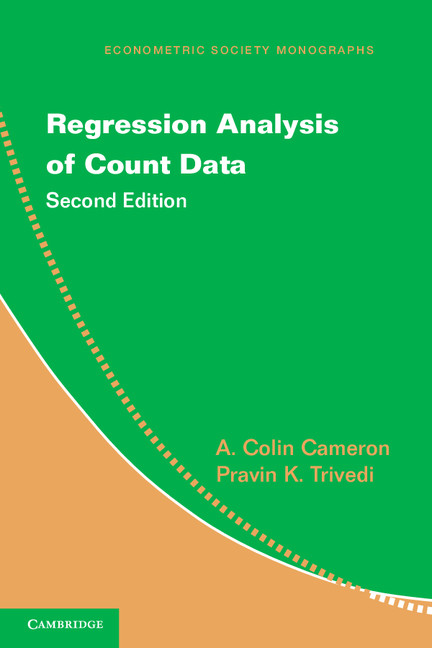
\includegraphics[width=.25\textwidth]{libro.png}
\end{figure}
Por ejemplo, el libro de \citeauthor{Cameron2013} \citeyear{Cameron2013} tiene casi 600 páginas que enseñan cómo aplicar modelos de regresión para casos de variables que no tienen una distribución normal (e.g., ventas).
\end{frame}

\begin{frame}
% \Large
Para ser exhaustivo al describir el comportamiento estadístico de una o más variables deberían señalarse sus valores de tendencia central (promedio, mediana, moda), dispersión (desviación estándar, varianza) y también los de forma (asimetría y curtosis) dentro de las tablas. \\
\vspace{0.5cm}
\centering
\pause
\textbf{¡Ese tipo de tablas son muy infrecuentes!}    
\end{frame}


\begin{frame}
\Large
Observemos esta tabla tomada de un paper sobre el ``secreto a la felicidad'' \cite{Tamir2017}
\begin{figure}
\centering
 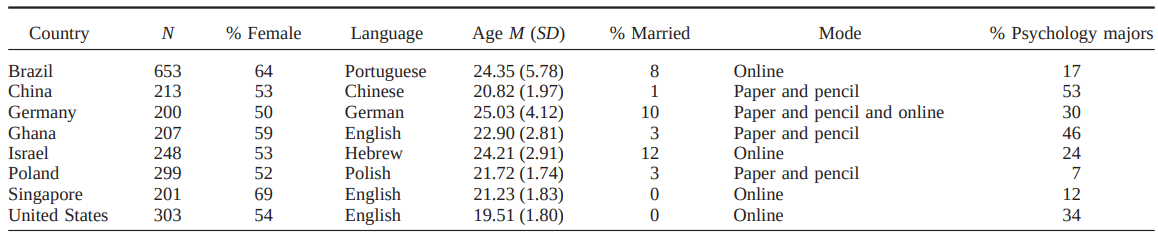
\includegraphics[width=1\textwidth]{Fig1}
\end{figure}
¿Y si comunicamos esta tabla pero con gráficos?
\end{frame}

\begin{frame}
\begin{verbatim}
\tiny
library(rworldmaps)\\
data("countryExData",envir=environment(),package="rworldmap")\\
sPDF <- joinCountryData2Map(countryExData, joinCode = "ISO3", nameJoinColumn = "ISO3V10")\\
mapCountryData(sPDF, nameColumnToPlot = ``Age'')
\end{verbatim}
\begin{figure}
\centering
 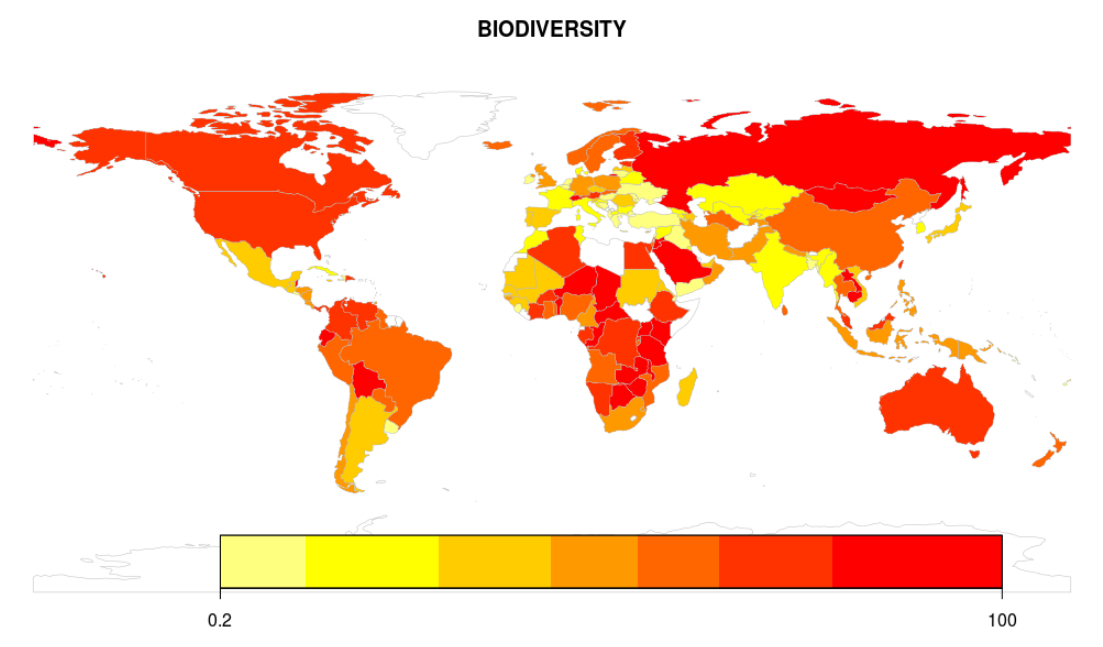
\includegraphics[width=0.6\textwidth]{Fig2}
\end{figure}
\tiny{Mapa generado con el paquete ``rworldmaps'' en el entorno R \cite{R2017}}
\end{frame}

\begin{frame}
\begin{figure}
\centering
 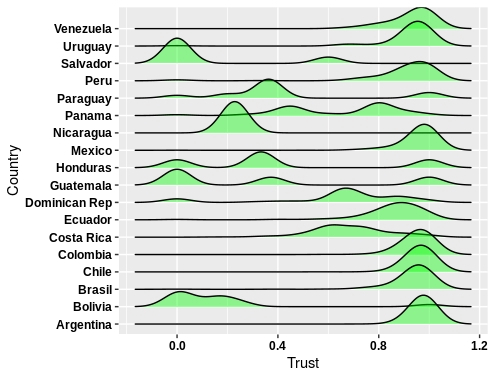
\includegraphics[width=0.6\textwidth]{Fig3}
\end{figure}
\end{frame}

\section*{REFERENCIAS}
\begin{frame}[allowframebreaks]{Referencias}
\tiny{ 
\bibliographystyle{apacite}
\bibliography{REFS.bib}
} 
\end{frame}

\setbeamertemplate{background}{\tikz[overlay,remember picture]\node[opacity=1]at (current page.center){
\includegraphics[width=18cm]{ulam.png}};}
\pgfdeclareimage[height=0cm,width=0cm]{}{}
 \logo{\pgfuseimage{}}
\beamertemplatenavigationsymbolsempty
\begin{frame}
\end{frame}
\end{document}